\documentclass[a4paper, 12pt]{article}
\usepackage[czech]{babel}
\usepackage[utf8]{inputenc}
\usepackage{graphicx}
\usepackage{float}
\usepackage[hang]{caption}
\usepackage[top=3cm, bottom=2cm, right=2.5cm, left=2.5cm]{geometry}
\usepackage{hyperref}
\usepackage{natbib}		
\usepackage{mathtools}
\usepackage{amsmath}
\bibpunct{(}{)}{;}{a}{,}{;}	

% --------<<< ------------------------- >>>--------

\begin{document}

\begin{center}
\textsc{Charles University} \\ 
\textsc{Faculty of Social Sciences}\\ 
\textsc{Institute of Economic Studies}\\[0.5em]
Data Processing in Python\\
SS 2022/2023\\ %[2em]
\end{center}

\begin{minipage}{1\textwidth}
\begin{center}
\title{\textbf{\emph{Project Report: 
Examination of Criminality in the Czech Republic based on Socio-Economic Determinants}}}
\author{\textbf{Tomáš Barhoň, Radim Plško}}
\date{August 2023}

\maketitle
\end{center}
\thispagestyle{empty}
\end{minipage}

\newpage %
\section{Introduction}
\paragraph{\normalfont{This report provides an overview of a project conducted by Tomáš Barhoň and Radim Plško for the Data Processing in Python class in the summer semester 2022/23. The project aims to study the impact of socio-economic indicators on the level of economic criminality in different regions of the Czech Republic ("obce s rozšířenou působností").}}

\section{Data Source}
\paragraph{\normalfont{The primary data source for this project is the https://kriminalita.policie.cz/ API, which provides information about various types of crimes and their precise geographical locations ("points of crimes"). Therefore, in order to be able to work with crimes on the level of regions ("ORP"), we needed to fit these points of crime to the geographical locations of ORPs. The socio-economic data were obtained from PAQ research and various open-data sources.}}

\paragraph{\normalfont{The socio-economic data were obtained from various open-data sources, but mainly from PAQ research (https://www.datapaq.cz/) where all data were recorded on ORP from the beginning which was the most convenient for us.}}

\paragraph{\normalfont{The study focused on the following four socio-economic indicators:}}

\begin{enumerate}
\item Lidé v exekuci (2021) - The percentage of people with foreclosure.
\item Podíl lidí bez středního vzdělání (2021) - The percentage of people without completed high school education.
\item Domácnosti čerpající přídavek na živobytí (2020) - The percentage of households receiving social benefits.
\item Propadání (průměr 2015–2021) - The percentage of children that obtain a grade of 5 from any subject at the end of the summer semester.
\end{enumerate}

\section{Crime Data}
\paragraph{\normalfont{The crime data was subset to meet specific conditions. The crimes included in the study are illegal, verifiable, and of an economic nature, such as thefts and burglaries - to be most relevant to the case of chosen specific socio-economic variables. The data was analyzed for the period from 2021 to 2023, yielding about 500,000 criminal records.}}

\newpage
\section{Code Overview}

\paragraph{\normalfont{The provided Python code begins with multiple import statements to load the necessary packages and modules essential for the data manipulation as pandas, numpy, json but also for data visualization as seaborn, visualizer, geopandas and folium.}}

\paragraph{\normalfont{After importing the necessary packages and modules, the code proceeds with the data processing. This includes:}}

\begin{enumerate}
\item the code initializes a "Downloader" class with specific parameters (e.g., year and month) to download criminal data from an API;
\item this data is then processed through the "Data\_pipeline" class, which matches the crime data to corresponding polygons using the "Region\_finder" module;
\item the number of crimes per polygon is computed, and the data is preprocessed before merging with other datasets;
\item the data is then merged into a final table, combining crime information with other relevant data, and the resulting table "DataFrame" contains structured information suitable for further analysis.
\end{enumerate}

\paragraph{\normalfont{The visualization is then done as follows (you can find described resulting images below at "Findings"). The "Visualizer\_of\_criminal\_data class" is initialized with the table DataFrame to create various visualizations of the criminal data. The code generates multiple interactive maps using the "folium" library, displaying different aspects of the crime data. The maps are stored in the "maps" list, and the corresponding English legend names are stored in the "labels" list. Each map is then displayed with its corresponding label using the "print()" function.}}

\newpage %
\section{Findings}

\paragraph{\normalfont{Firstly, we took a number of criminalities from the dataset, plotted in the ORPs and then plotted on the map using folium. As you can see, most of the crimes are in the big cities. This makes sense as there live more people. That is why we created a new variable and counted it per capita to make more sense. The results were still surprising for us as even per capita, most crimes were in Prague. Ostrava, Brno and Ústí nad Labem were the following cities with the largest number of crimes per capita.}}
\begin{center}
    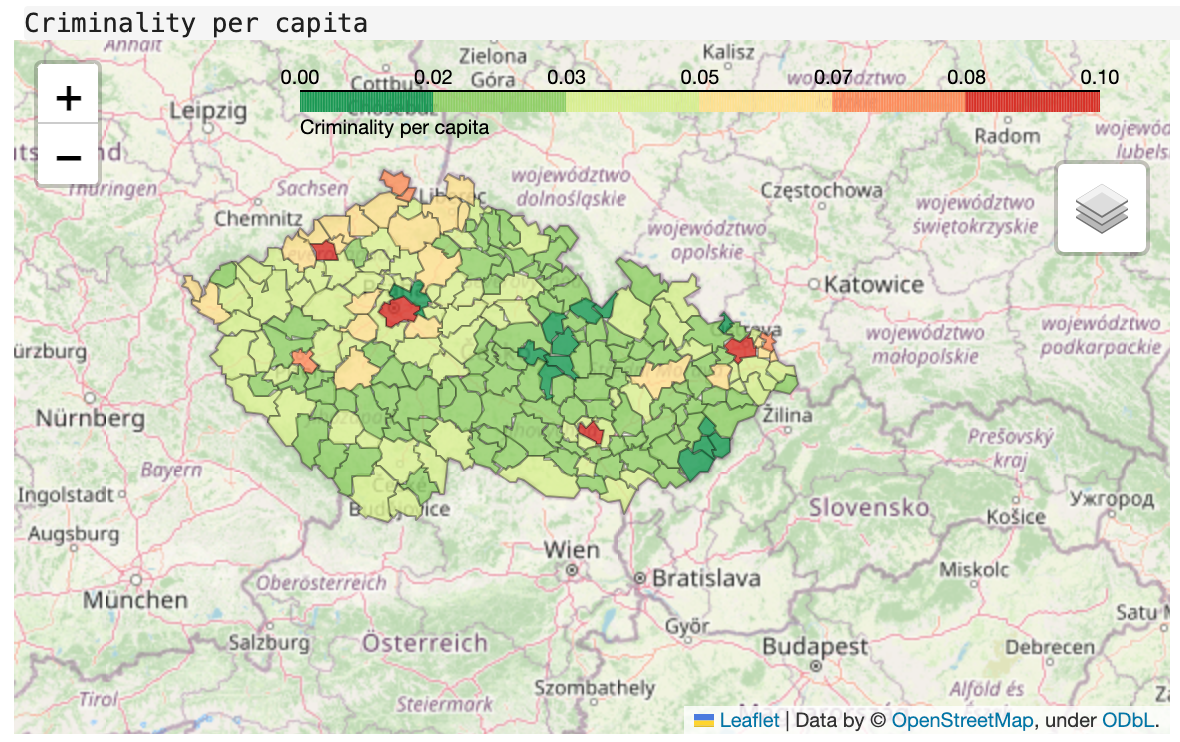
\includegraphics[width=.8\textwidth]{Criminality_per_capita.png}
\end{center}

\paragraph{\normalfont{Secondly, we plotted already mentioned socio-economic indicators with which we will work later, on the map to see a bigger picture of how these indicators result in each region before our later findings. You can see the results here.}}
\begin{center}
    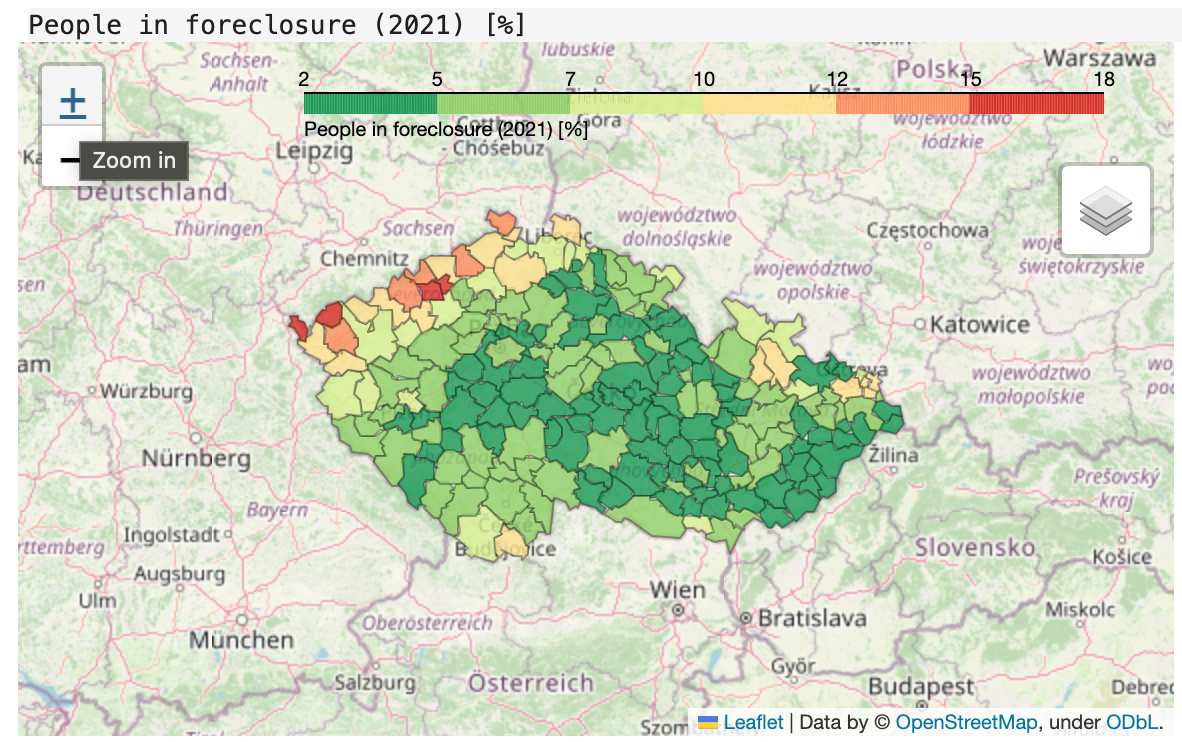
\includegraphics[width=.8\textwidth]{people_in_foreclosure.png}
    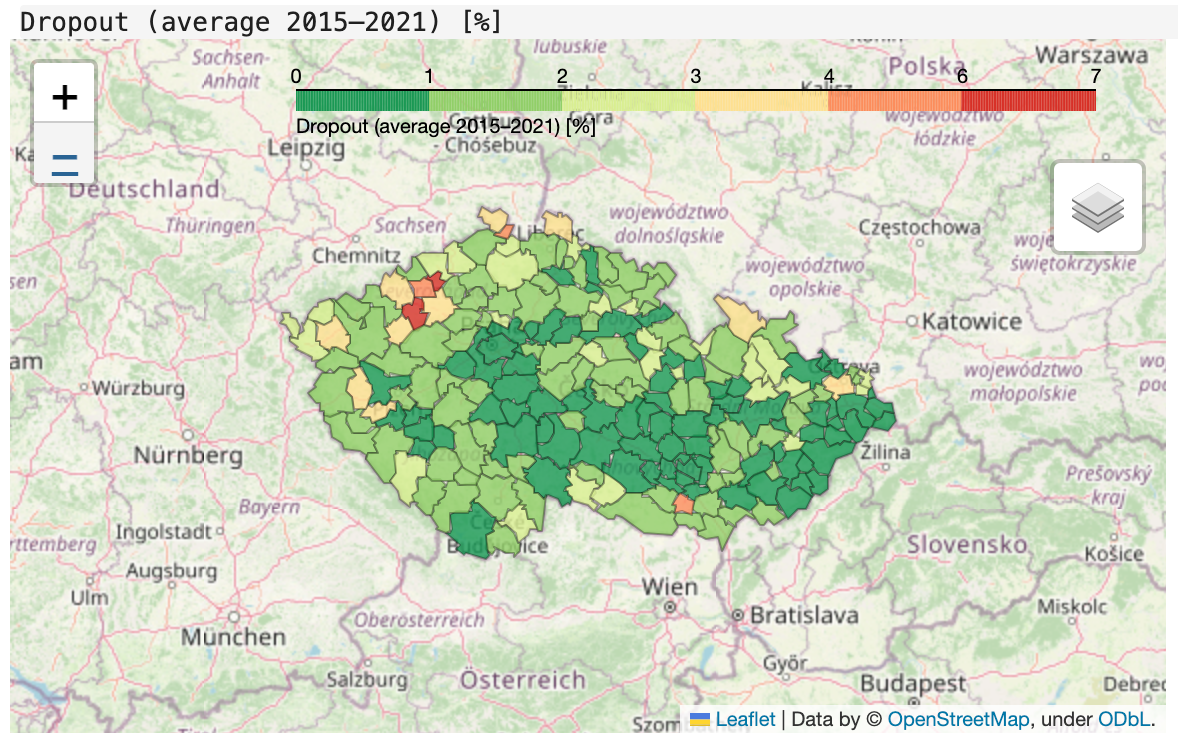
\includegraphics[width=.8\textwidth]{dropout.png}
    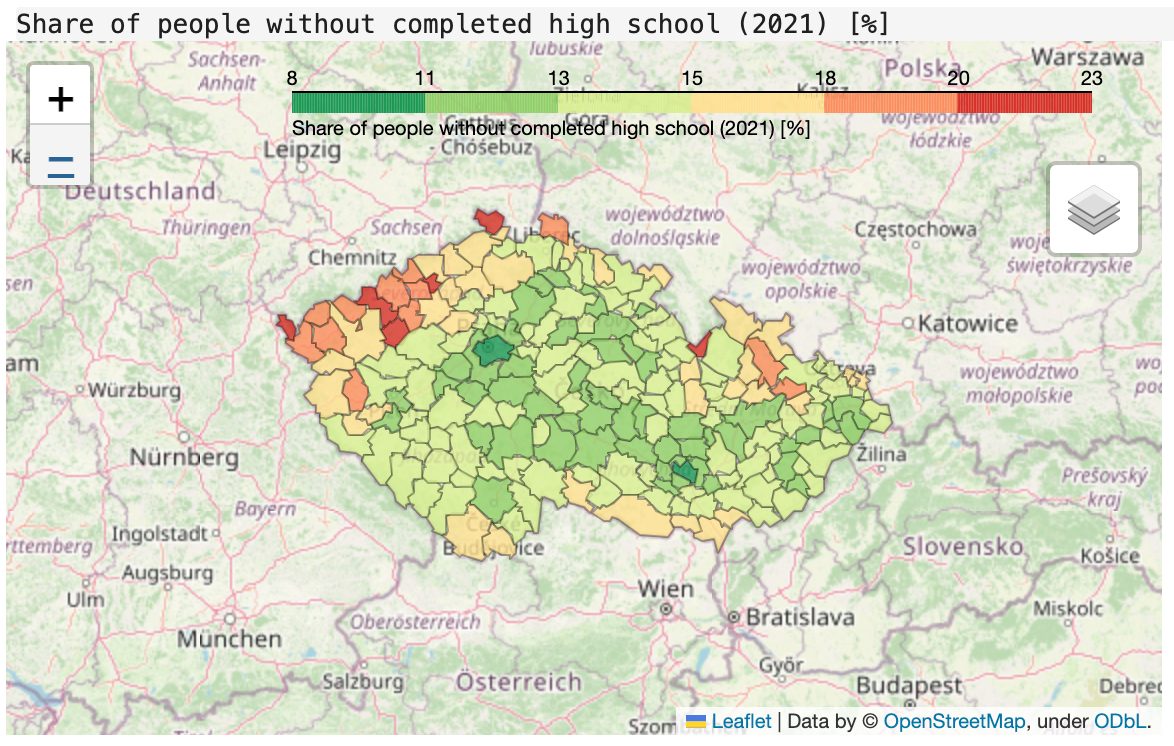
\includegraphics[width=.8\textwidth]{without_high_school.png}
       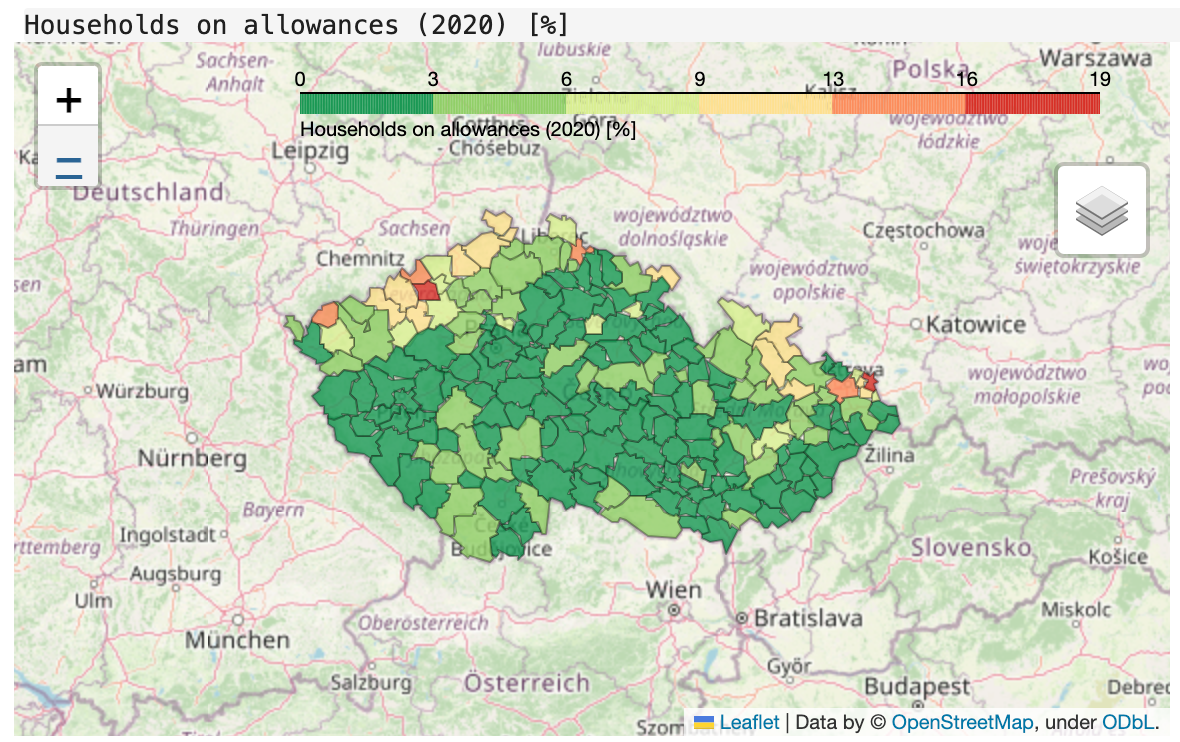
\includegraphics[width=.8\textwidth]{allowances.png}
\end{center}

\paragraph{\normalfont{Then, according to the procedure mentioned in "Code Overview" and which you can find on GitHub (https://github.com/Tomas-Barhon/Python-project), we used the data to create \textbf{Criminality risk index} that finally shows which ORPs are according to our analysis the most keen to economic crime acts. As you can see, the red area around Ústí nad Labem close to the German borders indicates a high rate of crimes. Ostrava and near cities follow as the second most criminal area in the Czech Republic. On the opposite, Prague or Brno, for example, came out as a safe space when we compare the findings to the initial maps. For all data we took for the criminality index, we took the number of inhabitants in the areas into consideration and count it per capita.}}
\begin{center}
    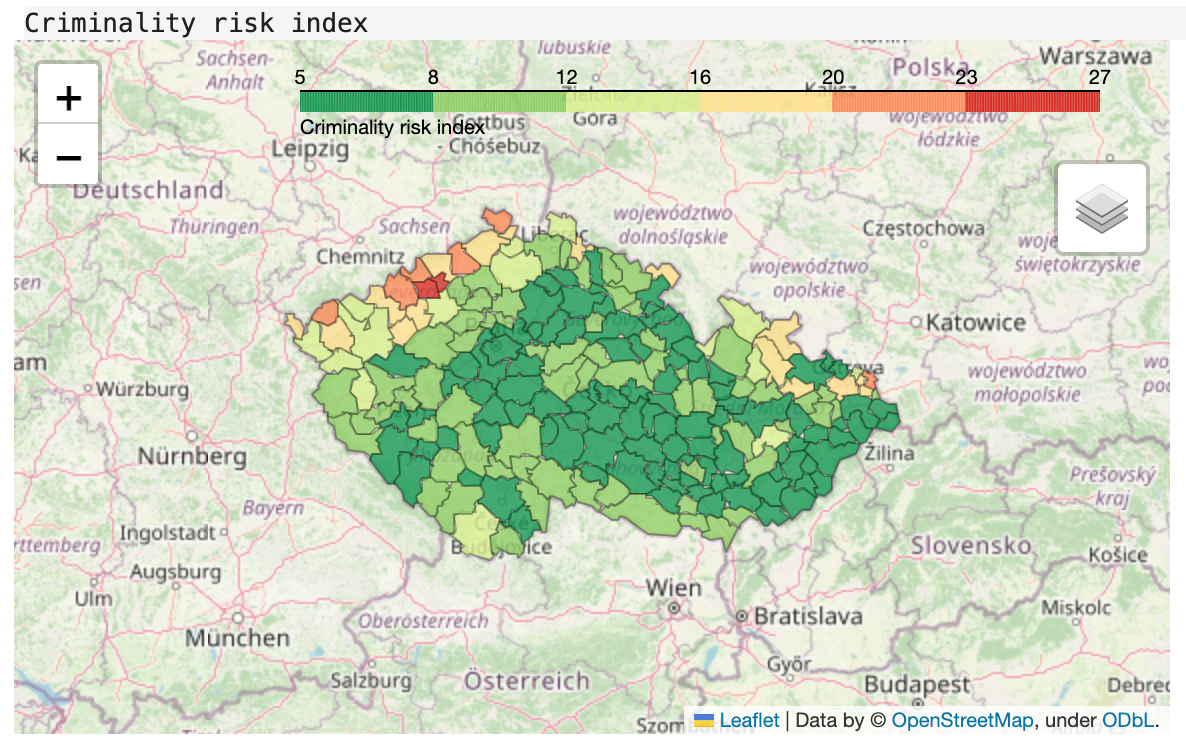
\includegraphics[width=.8\textwidth]{risk_index.png}
\end{center}

\paragraph{\normalfont{As a further analysis, we plot individual indicators on the correlation graph to really see how much these indicators correlate with the number of criminal activities per capita. You can see the graphs below.}}
\begin{center}
    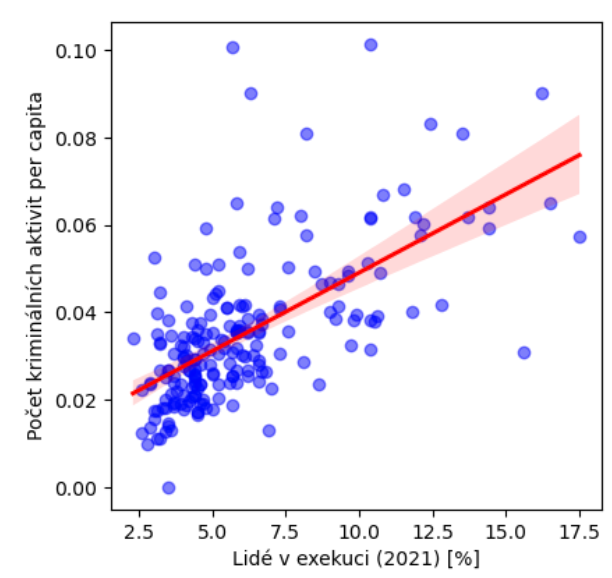
\includegraphics[width=.8\textwidth]{corr1.png}
    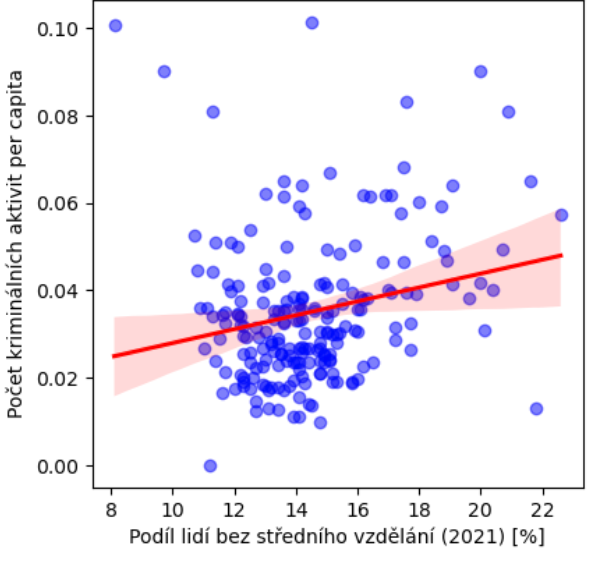
\includegraphics[width=.8\textwidth]{corr2.png}
    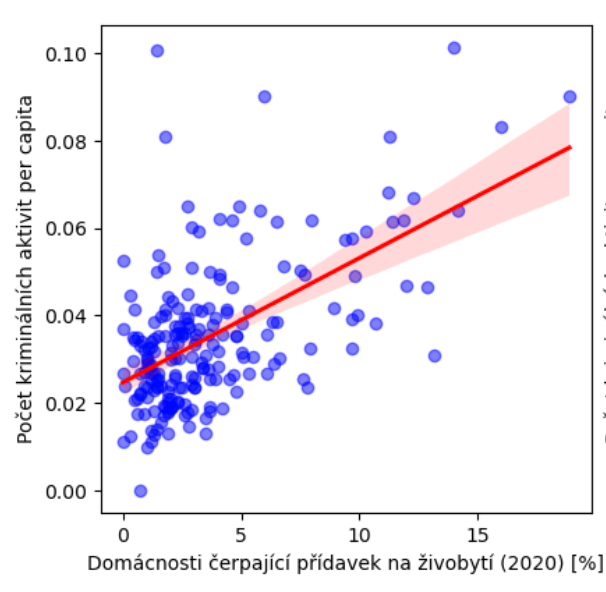
\includegraphics[width=.8\textwidth]{corr3.png}
    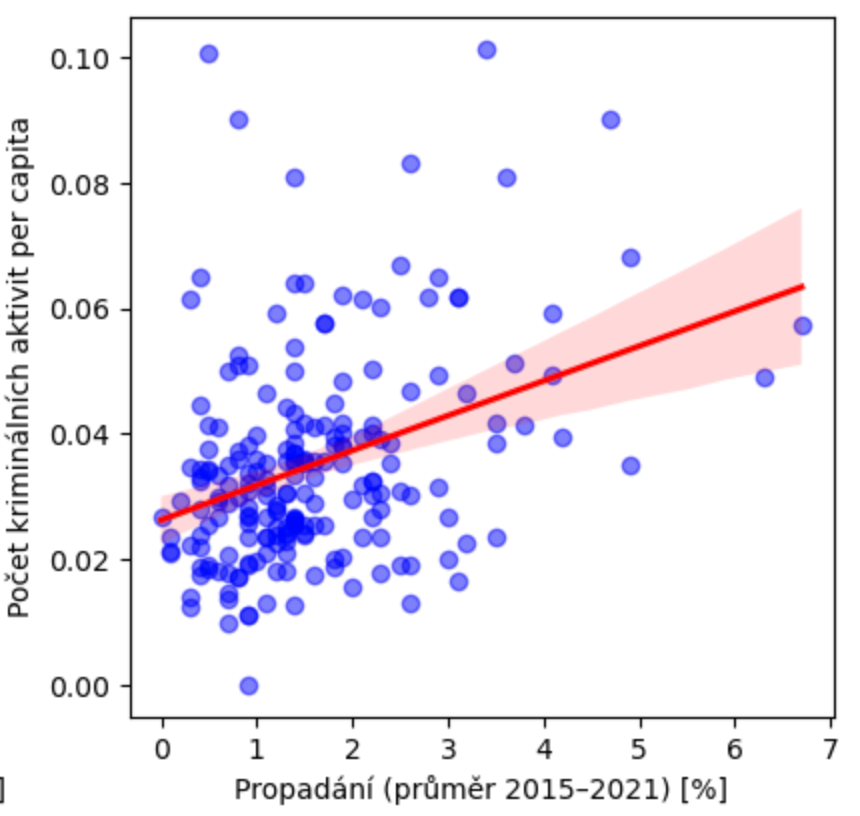
\includegraphics[width=.8\textwidth]{corr4.png}
\end{center}

\paragraph{\normalfont{As you can see, the most correlated with the number of criminal activities per capita is "The percentage of people with foreclosure" (0.63) and "The percentage of households receiving social benefits" (0.57) which are almost of the same correlation. On the other hand, the least correlated is "The percentage of people without completed high school education" (0.22) which does not influence the number of criminality in the regions as much - it also has the biggest deviation of the all mentioned indicators (which makes sense). Exact correlation numbers are visualized below on the correlation scale.}}
\begin{center}
    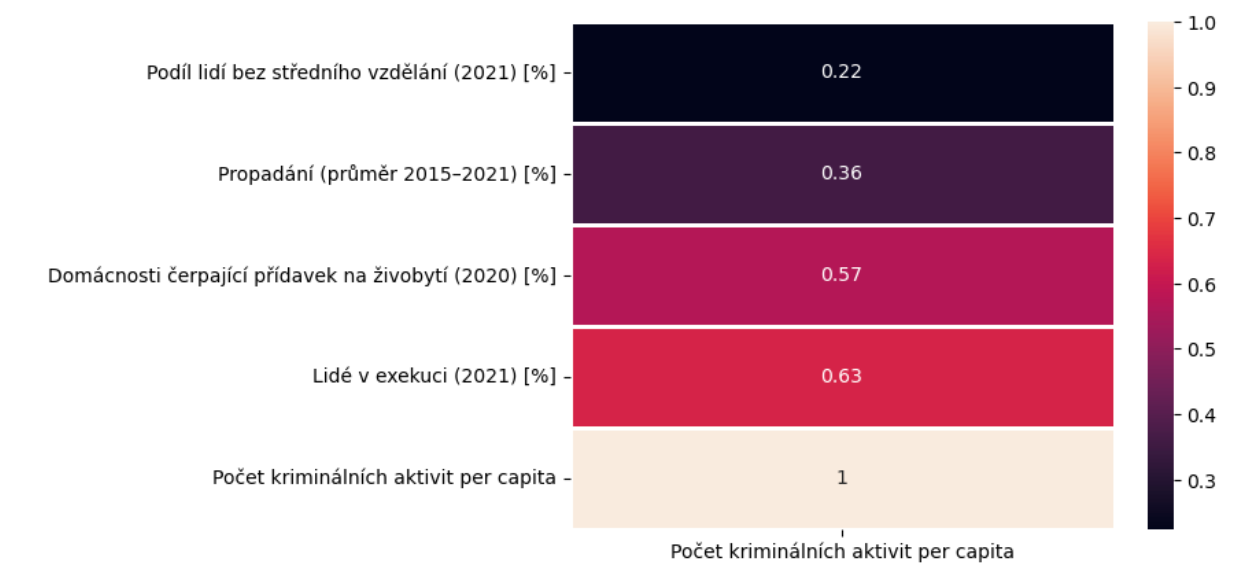
\includegraphics[width=.8\textwidth]{corr_index.png}
\end{center}

\section{References}
\paragraph{\normalfont{The data used in this project, that we acquired from PAQ research, were obtained from various sources including the Czech Statistical Office, the Agency for Social Inclusion, the Ministry of Labour and Social Affairs, the Chamber of Executors of the Czech Republic, and the Czech Household Panel Study.}}

\paragraph{\normalfont{The records of crime acts are exclusively from the Police of the Czech Republic which as the only one has the resources for it. }}

\bibliographystyle{apa}
\bibliography{bibliography.bib}	

\end{document}